Using the 313 nm laser, we fluoresce the \ce{Be+} ions and cool them down to a cloud or crystal in the ion trap. The scattered light is observed via our imaging system shown in Figure \ref{fig: imaging system}. The components include the Andor iXon3 camera with EM gain, a 313 nm band pass filter, angled mirror, enclosing lens tubes, and Sill objective lens with 0.2 NA, and 40 mm working distance. The alignment of our objective lens to camera imaging plane yields a magnification of about $\times5.5$. All of the imaging components are rigidly mounted onto the 3 axis translation stage allowing us to move the focal point without changing the magnification. The total efficiency of our imaging system is
\begin{equation}
	\epsilon = \Omega \alpha \beta \gamma
	\label{eq: fluorescence efficiency}
\end{equation}
where $\Omega$ is the solid angle the reentrant objective appends, $\alpha$ is the camera's quantum efficiency at 313 nm, $\beta$ is the camera's exposure time, and $\gamma$ is the camera's gain. For a fluorescing ion scattering at $\Gamma \times (\rho_{pp} \approx 0.20)$, we expect on the order of $10^5$ counts per ion after the imaging inefficiencies.

With images of the ion clouds used in our chemical reaction studies, approximate the temperature of the ions by assuming they are in a harmonic potential. In the same fashion that we derived the trap depth, we may find a characteristic temperature of the ion cloud in the trap from the spacial width. With a very large cloud of ions that are not in a Coulomb crystal, we estimate a maximum temperature of 500 mK by estimating the physical width of the ion cloud. When compared to the temperature of a gas introduced via leak valve or even the CBGB, the ions in the trap may be considered to effectively have zero velocity.

\begin{figure}[H]
	\centering
	\includegraphics[height=0.8\textwidth]{images/imaging_system.jpg}
	\caption{The Andor iXon3 camera, enclosed imaging pathway, and objective lens are all mounted onto a 3 axis translation stage. The Sill objective lens is mounted at then end of the imaging tubes, inserted into the reentrant flange. An angled mirror directs the light at a 90$^\circ$ angle up and through a 313 nm bandpass filter placed in front of the camera sensor.}
	\label{fig: imaging system}
\end{figure}

\begin{figure}
	\centering
	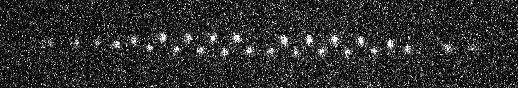
\includegraphics[width=0.8\textwidth]{images/ion_crystal.png}
	\caption{Laser cooled Coulomb crystal of \ce{Be+} ions in the LQT imaged with the reentrant imaging system. Dark \ce{BeH+} ions are sympathetically cooled in the middle of the top row as well as the third position from the right.}
	\label{fig: ion crystal}
\end{figure}